\chapter{Relatório quantitativo} %Apêndice C
\label{apendice:c_relat_quantitativo}

Este apêndice apresenta um relatório composto dos resultados das questões objetivas do questionário de coleta de dados.
\section{Quanto ao perfil dos respondentes}
Em um total de 53 participantes, o gráfico abaixo apresenta a proporção dos cargos efetivos dos servidores participantes da coleta de dados.

\begin{figure}[h]
\centering % para centralizarmos a figura
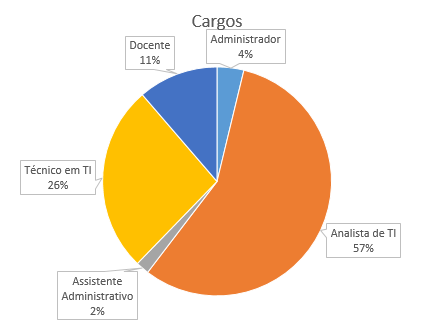
\includegraphics[width=9cm]{figuras/apendiceC_cargos.png}
%\caption{Cargos dos respondentes.}
\end{figure}

Dos 53 participantes, 34 possuem cargo de confiança.

Com relação ao tempo na instituição (em anos), os participantes se distribuem da seguinte forma:
\begin{itemize}
\item 2 anos ou menos: 9 participantes;
\item 3 a 5 anos: 22 participantes;
\item 6 a 10 anos: 14 participantes;
\item 10 a 20 anos: 5 participantes;
\item 20 anos ou mais: 3 participantes.
\end{itemize}

Com relação à formação acadêmica, os participantes estão distribuídos da seguinte forma:
\begin{figure}[h]
\centering % para centralizarmos a figura
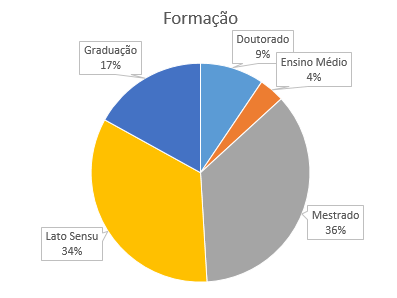
\includegraphics[width=9cm]{figuras/apendiceC_formacao.png}
%\caption{Formação dos respondentes.}
\end{figure}

\section{Quanto ao PDTI}
\begin{itemize}
\item Afirmaram possuir PDTI: 81\% (30 instituições)
\item Afirmaram não possuir PDTI: 19\% (7 instituições)
\end{itemize}

Este resultado se difere dos números do TCU em seu levantamento com 355 órgãos federais \cite{tcu:14}, dos quais 33\% afirmaram não possuir PDTI. Esta diferença sugere que no caso específico de instituições de ensino federais o nível de aderência ao planejamento de TI é melhor do que o percentual geral envolvendo os demais órgãos federais. Porém, é importante ter cautela ao tirar conclusões. Um estudo focado em comparar as instituições de ensino com as demais instituições federais poderia esclarecer as razões desta diferença.

%Foi possível extrair uma visão quantitativa das dificuldades encontradas pelos respondentes que participaram da elaboração do PDTI das suas respectivas instituições. 
No questionário foi perguntado acerca do grau de dificuldade na realização de algumas atividades essenciais no planejamento de TI, o grau de dificuldade poderia variar de 0 (nenhuma dificuldade) a 10 (muita dificuldade). Na figura abaixo é possível inferir que as maiores dificuldades na fase de levantamento de necessidades estão nas atividades de identificação das necessidades de informação e, principalmente, na definição de critérios de priorização das necessidades levantadas. 
\begin{figure}[h]
\centering % para centralizarmos a figura
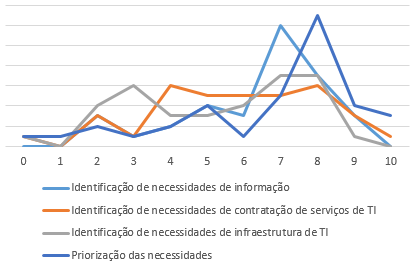
\includegraphics[width=9cm]{figuras/grafico_dificuldades.png}
%\caption{Formação dos respondentes.}
\end{figure}

Foi perguntado para os respondentes do grupo de instituições que possui PDTI se eles seguiram o Guia do SISP (modelo de elaboração do PDTI). Os números absolutos são distribuídos como segue:
\begin{itemize}
\item Não usaram o Guia do SISP: 3 participantes;
\item Usaram o Guia do SISP parcialmente: 12 participantes;
\item Usaram o Guia do SISP completamente: 21 participantes;
\item Não souberam informar: 1 participante.
\end{itemize}

Utilizando a escala de 1 a 5, onde 1 corresponde à "discordo totalmente" e 5 à "concordo totalmente", foi perguntado aos participantes se eles concordam que no PDTI das suas respectivas instituições havia determinados elementos. O gráfico abaixo apresenta a percepção dos participantes sobre a presença destes elementos no PDTI.

\begin{figure}[h]
\centering % para centralizarmos a figura
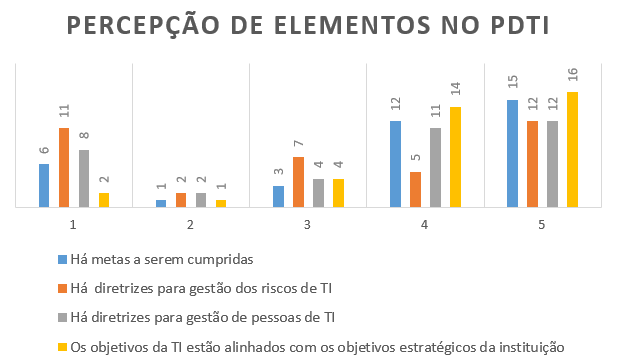
\includegraphics[width=11cm]{figuras/apendiceC_percepcaoelementos.png}
%\caption{Formação dos respondentes.}
\end{figure}
